\documentclass{rbf}
%\documentclass[onecolumn]{rbf}
\usepackage[T1]{fontenc}
\usepackage{graphicx}
\graphicspath{{circuito__y_componentes/}}
\begin{document}
\title{ESTUDIO DINÁMICO EN CIRCUITOS CAÓTICOS MEDIANTE \\EXPERIMENTOS SIMULADOS,  NUMÉRICOS Y FÍSICOS}

\author{A. Alejandro S. Coro\marca{\dag}}
\afil{\marca{\dag} Carrera de física\\ 
Facultad de ciencias puras y naturales\\
Universidad Mayor de San Andrés\\
La Paz - Bolivia}
\alpie{\dag}{Email: asuxoc@fcpn.edu.bo.}\\

\begin{abstract}
\Resumen
Se realizo un estudio dinámico mediante experimentos simulados, numéricos y físicos, de un circuito caótico modificado propuesto tipo Chua. Comparamos cualitativamente los resultados con una vasta galería atractores y, para un caso, se verifican sus comportamientos dinámicos cuantitativamente mediante los exponentes de Lyapunov y el parámetro d-infinito. Estos resultados están en concordancia con el trabajo de Conde-Ramírez(2007) y Gallas-Ramírez(2008), solo que aquí, se enfoco sobre todo en la influencia de valores elevados en la resistencia interna del inductor el circuito de Chua y como puede ser solventada con una modificación que, de cierta manera, introduce histéresis. 
\descriptores{Caos determinista - circuitos caóticos - histéresis - exponentes de Lyapunov - tiempo de simulado en regiones transitorias y asintóticamente estables.}
\pacs{05.45.\_a, 05.45.Xt}

\Abstract 
A dynamical study was carried out by simulations and physical experiments, of a proposed modified chaotic circuit of the Chua type. We qualitatively compare the results with a vast attractor gallery and, for one case, we verify quantitatively by means of the Lyapunov exponents and the d-infinite parameter. These results are in agreement with the work of Conde-Ramírez(2007) and Gallas-Ramírez(2008). Additionally we proceed to experimentally couple two of these circuits and only the gallery is shown.

\keywords{Deterministic chaos - chaotic circuits - hysteresis - Lyapunov exponents - transient and asymptotically stable regions.}
\end{abstract}

\shortauthors{A. Alejandro S. C.}
\shorttitle{EXPERIMENTOS SIMULADOS, NUMÉRICOS Y FÍSICOS EN CIRCUITOS CAÓTICOS}
\PrimPag{1}
\volumenyanio{n}{2022}

%\maketitle

\section{Introducción}
%\verb+\title{#1}+ para que la letra salga tal cual.
El estudio de circuitos caóticos es muy importante no sólo para comprender la naturaleza del caos, sino también para desarrollar aplicaciones sofisticadas que utilicen realmente este comportamiento. En vista de la emocionante aparición de la nanotecnología, encriptación de información basada en el caos y el atractivo futuro de la computación cuántica, los circuitos no lineales se han vuelto aún más importantes y fundamentales. Esto requiere una investigación exhaustiva de las características dinámicas y los mayores regímenes de supervisión posibles de circuitos y sistemas no lineales. 

\begin{figure}
    %\centering
    \includegraphics{circuito de Chua.png}
    \caption{\label{fig:circuito de Chua}Circuito de Chua utilizando dos amplificadores operacionales (op amps) y seis resistencias lineales que están disponibles en un único circuito integrado de ocho pines (TL082), que forma el diodo de Chua $N_{R}$ implementado por Kennedy (1992).}
\end{figure}

\subsection{Circuito de Chua clásico y modificado}
El circuito de Chua (CC), se muestra en la 
Fig. \ref{fig:circuito de Chua}, es uno de los modelos más populares que exhiben caos puesto que es el circuito autónomo más simple capaz de mostrar comportamiento caótico. Está compuesto por una parte que presenta un comportamiento típico de un oscilador amortiguado (dos condensadores $C_1$ y $C_2$, una resistencia variable R y una bobina L) y la otra parte que constituye el único elemento no lineal denominado diodo de Chua $N_R$ que básicamente es una resistencia no lineal o lineal por partes (Piecewise linear o PWL) como se muestra en la Fig \ref{fig:diodo teórico}. Este elemento causante de la no linealidad actúa como la fuente de energía de todo  el circuito, se ocupa de retroalimentarlo y lo mantiene oscilando.

Escribiendo las variables dinámicas $V_{C1}$, $V_{C2}$ e $I_L$, junto con los voltajes de quiebre $-B_{p}$ y $+B_{p}$, como:
\begin{eqnarray}\label{x y z adimensionales}
    \begin{split}
        x=V_{C1}/B_p,\\
        y=V_{C2}/B_p, \\
        z=RI_L/B_p, \\
        \tau=t/RC_2
    \end{split}
\end{eqnarray}
se obtiene las ecuaciones diferenciales adimensionales del CC:
\begin{eqnarray}\label{Chua eq dif}
    %\centering
    \begin{split}
    dx/d\tau &= \alpha(y - x - f(x))\\
    dy/d\tau &= x-y+z\\
    dz/d\tau &= -\beta y -\gamma z\\ 
    \end{split}
\end{eqnarray}
y
\begin{eqnarray}\label{alfa beta gamma}
\begin{split}
    \alpha&=C_{2}/C_{3}\\
    \beta&=R^{2}C_2/L\\
    \gamma&=r_{0}RC_{2}/L
\end{split}
\end{eqnarray}
Donde se añadió la resistencia lineal $r_0$ en serie con el inductor en el esquemático de la Fig.\ref{fig:circuito de Chua}, esto se conoce como el circuito de Chua canónico (CCC) en el sentido de que puede exhibir todos los posibles fenómenos dinámicos asociados con cualquier vector de campo continuo lineal a trozos simétrico de tres regiones. En el caso que no se considera la resistencia $r_0$, el valor de $\gamma$ es nulo y el circuito se convierte en el caso simple/ideal donde no se considera resistencia interna en el inductor. 
La función PWL que describe el comportamiento del diodo de Chua, es:
\begin{equation} \label{f(x) PWL}
    f(x) = m_{0}x + 1/2(m_{1}-m_{0})(|x+B_p|- |x-B_p|)\\
\end{equation}
y las pendientes se pueden escribir como:
\begin{eqnarray}\label{pendientes}
    %\begin{split}
        m_0=R(-1/R_3 +1/R_4)\\
        m_1=R(-1/R_3 -1/R_6)
   % \end{split}
\end{eqnarray}
$m_{1}$ y $m_{2}$ son las pendientes negativas de la Fig.\ref{fig:diodo teórico}.

\begin{figure}
    \centering
    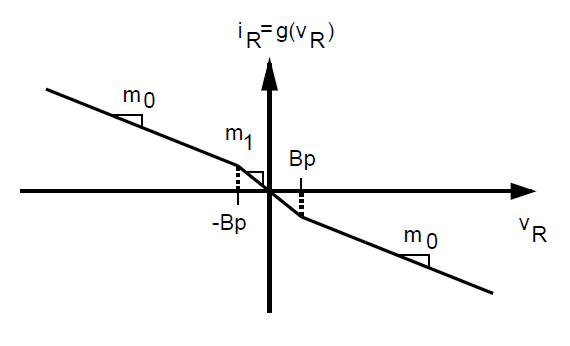
\includegraphics[width=7cm,height=7cm]{DiodoChua.png}\\
    \caption{Relación Corriente Voltaje del Diodo de Chua. $-B_{p}$ y $+B_{p}$son los puntos de quiebre de la relación corriente voltaje del diodo de Chua, mientras que $m_{0}$ y $m_{1}$ son las pendientes de la región externa e interna, respectivamente.} 
    \label{fig:diodo teórico}
\end{figure}

Después del advenimiento del circuito caótico de Chua, se han reportado numerosos trabajos sobre diferentes esquemas de realización de este circuito. Pues, es atractivo buscar un circuito de Chua actualizado que tenga comportamientos dinámicos similares al circuito clásico de Chua, pero que posea una estructura topológica de circuito mucho más simple (si se puede con un comportamiento dinámico más complejo) y sea mucho más fácil de implementar en la práctica. Todas estas realizaciones se centran principalmente en dos propósitos: realización sin inductor del circuito de Chua y realización del diodo de Chua basada en componentes electrónicos listos para usar. Generalmente, la razón detrás de la realización sin inductor radica en el hecho de que la presencia de un inductor de bobinado manual con resistencia parásita hace inadecuado el diseño de circuitos integrados y en muchas ocasiones no se pueda implementar. He aquí, donde nuestra propuesta entra en acción.
En 1990, Murali y Lakshmanan exploraron el circuito de Chua autónomo con una excitación externa periódica que convierte al circuito en no autónomo. Observaron una inmensa variedad de secuencias de bifurcaciones, histéresis y la coexistencia de múltiples atractores. Pero, sin modificar el diodo de Chua. Lindberg en 1992, en base al trabajo de Murali y Lakshmanan realizo una explicación sencilla del comportamiento físico del circuito y verifico mediante simulación algunas de las conclusiones de Murali y Lakshmanan, pues las imágenes y demás detalles reportados no están muy claros.
Por un lado, el circuito de Chua, a pesar de su simplicidad, permite observar muchos comportamientos dinámicos tomando una característica lineal por partes; posteriormente, también se desarrolló una versión aproximada con una no linealidad cubica.
Por otro lado, Makoto y Chua (2004) generaron osciladores no lineales histeréticos con diodos de Chua, i.e., utilizaron distintas configuraciones en circuitos con el diodo de Chua (sin modificarlo) junto con otros componentes electrónicos (capacitores, inductores, etc.) y producían fenómenos de histéresis. Dicho estudio, surgió debido a que en otros circuitos caóticos utilizaron la histéresis como elemento no lineal, como el circuito de Saito (1990). Flores (2008) asevera: "A diferencia del circuito de Chua, el circuito de Saito no ha tenido la suficiente atención que requiere, pero no hay duda de que en los próximos años sea uno de los circuitos más estudiados, ya que este circuito presenta un comportamiento hipercaótico."
La no linealidad de la histéresis es ampliamente exhibida en una variedad de materiales y sistemas. Thompson y Steward definen el fenómeno de histéresis como:
“El fenómeno, generado por una bifurcación catastrófica-peligrosa, en el que una trayectoria atractora no se restablece (inmediatamente) al invertirse el barrido de control. Dos bifurcaciones de este tipo suelen generar un bucle de histéresis, que se observa, por ejemplo, durante los barridos de frecuencia a través de la resonancia no lineal.”

Aquí se propone una modificación del CCC que lleva a ver un fenómeno de histeresis asociado al comportamiento no lineal del diodo de Chua.

En el presente trabajo, en la sección (2) utilizando resistencias internas elevadas del inductor se propone una modificación del CCC, que de una manera simple, introduce histéresis. Se realiza una comparación cualitativa de los comportamientos obtenidas para el CCC con resistencias elevadas y con la modificación propuesta, realizando simulaciones con el software de circuitos eléctricos LTSpice XVII.

En la sección (3) se compara los resultados de la simulación del CCC con resistencias elevadas con resultados numéricos de las ecuaciones del CCC bajo los mismos valores de los componentes electrónicos. 
También, se caracterizan algunos comportamientos utilizando los exponentes de Lyapunov y el parámetro d-infinito. Para este caso numérico se utiliza una aproximación cubica para la función PWL como se hace en el trabajo de Gallas-Rámirez. Y en la sección (4) se muestran los comportamientos dinámicos obtenidos de experimentos físicos del circuito con el CCC modificado. 

Adicionalmente procedemos a acoplar experimentalmente dos CCC modificados y solo se muestra la galería de atractores en la sección de anexos.

\begin{figure}
    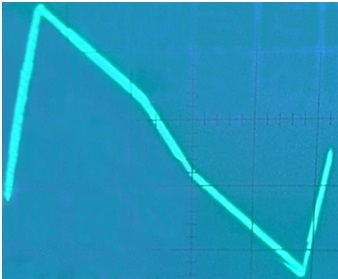
\includegraphics[width=3.9cm,height=3.9cm]{Fotos_Chua_Experimentales/DiodoSinModChua.jpg} & 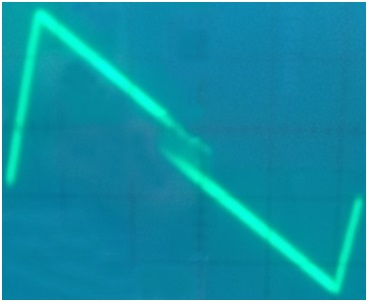
\includegraphics[width=4cm,height=4cm]{Fotos_Chua_Experimentales/DiodoModChua.jpg}\\
     (a) & (b) \\
    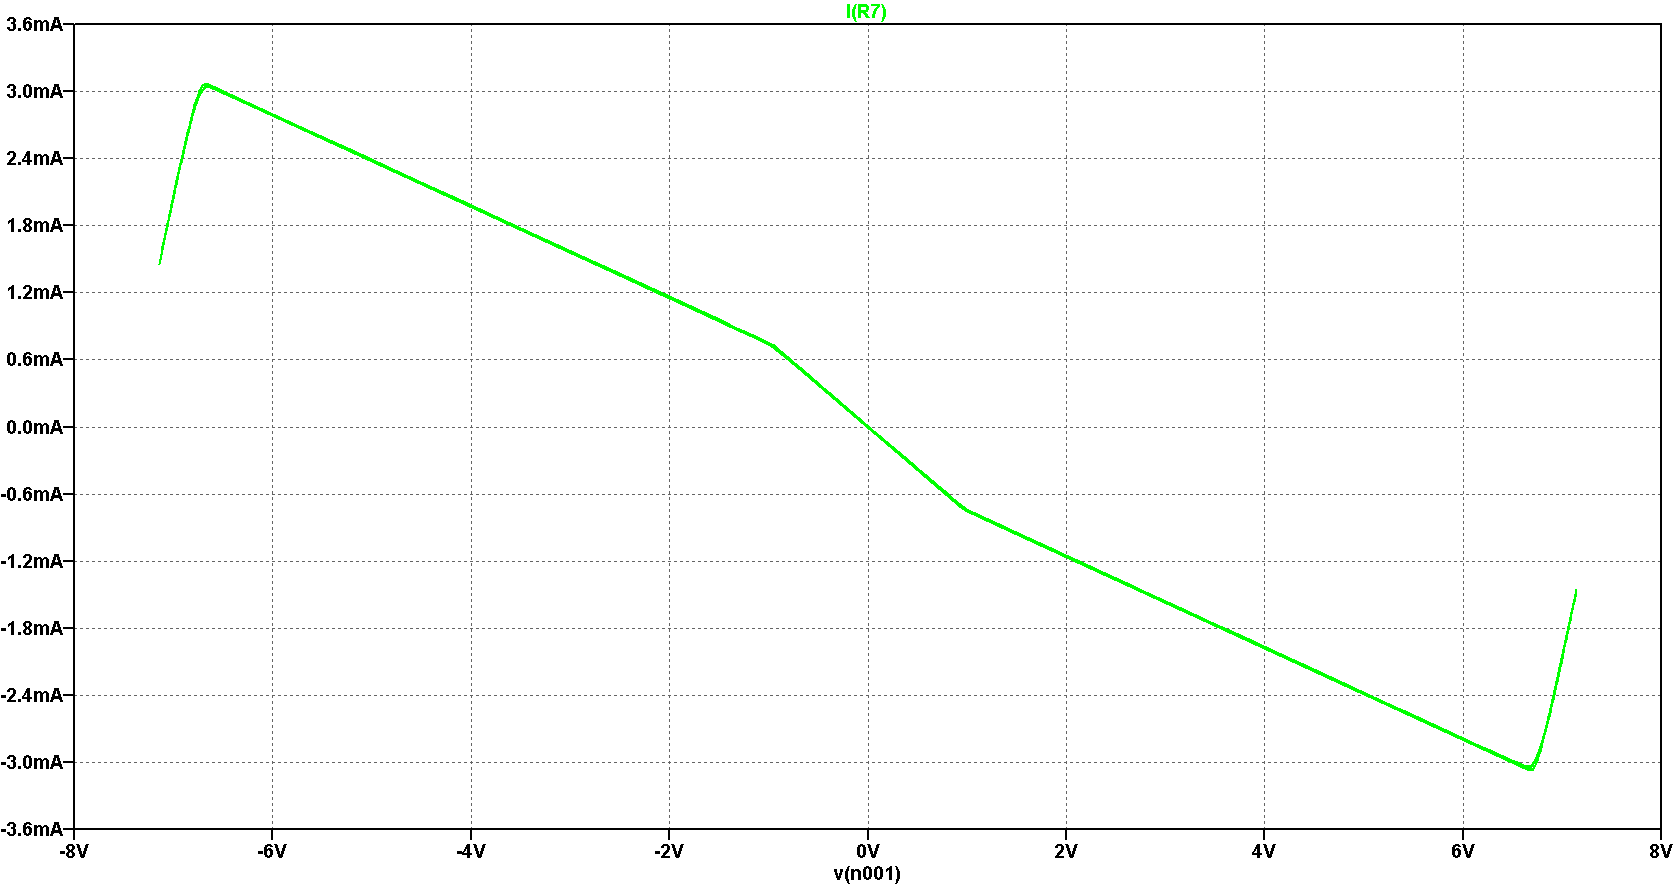
\includegraphics[width=4cm,height=4cm]{diodoPWL LTSpice.png} & 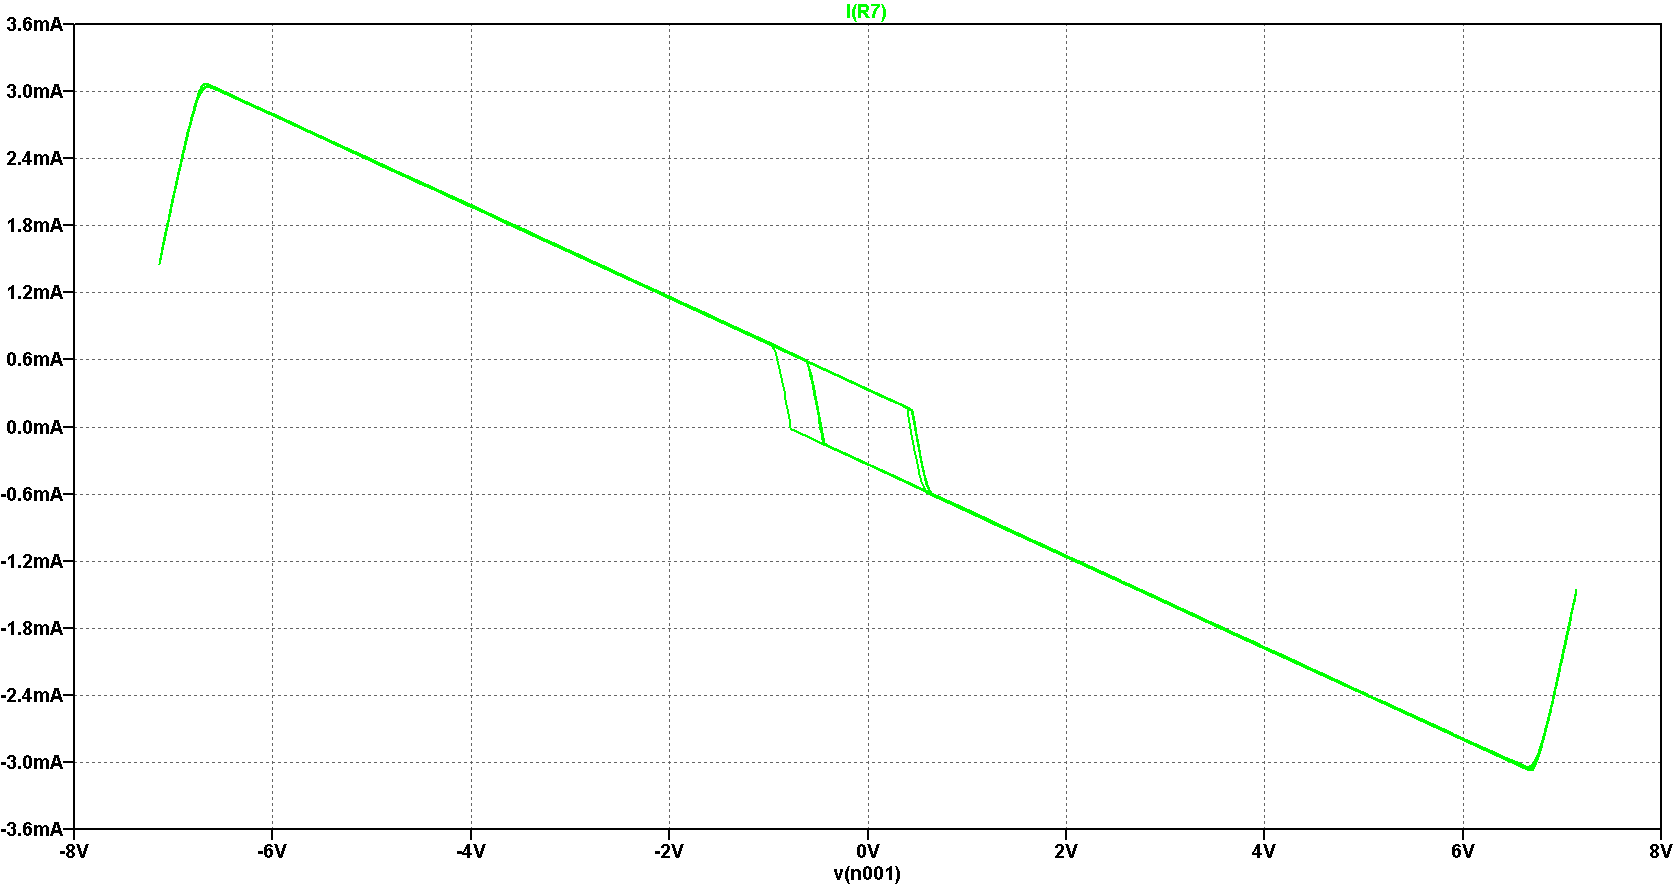
\includegraphics[width=4cm,height=4cm]{diodoPWL histeresis LTSpice.png}\\
     (c) & (d) \\     
    \caption{\label{fig:diodos experimentales} Comportamiento no lineal del diodo de Chua y su modificación: en osciloscopio (a) PWL y (b) PWL con histeresis en la parte central. En simulaciones: (c) PWL y (d) PWL con histeresis en la parte central.}
\end{figure}

\section{CCC modificado\label{sec:Circuito de Chua modificado}}

\begin{figure}[h]
    \centering
        \hspace{0cm}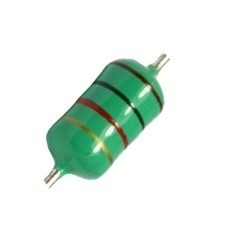
\includegraphics[width=4cm,height=3cm]{InductorMoldeado.jpg}\\
         (a)\\
        \hspace{0cm}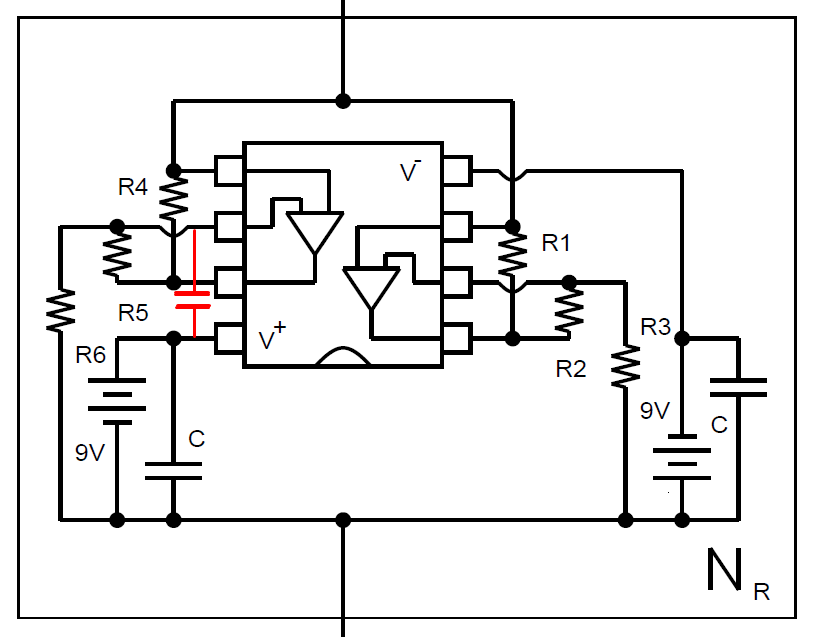
\includegraphics[width=6cm,height=5cm]{diodo modificado.png}\\
         (b)\\
    \caption{ (a)Esquemático del diodo de Chua modificado con un condensador cerámico en los terminales 6 y 8 (color rojo) del circuito integrado TL082. (b) Inductor moldeado, de fácil adquisición.}
    \label{bobina o inductor moldeado y diodo modificado}
\end{figure}

Para ver una nueva dinámica o identificar mejor la dinámica oculta del circuito de Chua, es significativo diseñar un diodo de Chua lineal por partes con los segmentos deseados, Wang et. al. (2019) utilizaron un diodo lineal a trozos de 5 segmentos para ver nuevos atractores y Medrano et. al. (2004) utilizaron un diodo de Chua modificado para identificar atractores ocultos y atractores coexistentes. En estos y muchos otros trabajos se puede ver que varios autores modifican dicho circuito de alguna manera según las necesidades requeridas.

La propuesta del CCC modificado ($C^3$M), se realiza utilizando un inductor de elevada resistencia interna parásita(Fig. \ref{bobina o inductor moldeado y diodo modif}(a)) y alterando el funcionamiento del diodo de Chua, i.e., sin los condensadores C de derivación conectados a cada batería de 9V, cuyo propósito es mantener las fuentes de alimentación con una tensión continua, y con la adición de un capacitor en las terminales 6 y 8 del circuito integrado (que esta en color rojo) en la Fig. \ref{bobina o inductor moldeado y diodo modificado}(b). 

Realizando estas modificaciones el diodo de Chua ya no es lineal en la parte central y se convierte en un bucle de histeresis. 
El comportamiento lineal a tramos del diodo de Chua se muestra en la Fig.\ref{fig:diodos experimentales}(a), el comportamiento del diodo de Chua modificado con una “histéresis” en la parte central se muestra en la Fig.\ref{fig:diodos experimentales}(b).

Recalcando nuevamente que, esta modificación sirve para que ¡el CCC pueda funcionar! con una resistencia parásita interna elevada del inductor, superior a 30 $(\Omega)$ segun el criterio de Siderskiy. La mayoría de CCC no funciona con este tipo de inductores, ya que están diseñados con inductores de resistencia parásitas interna bajas, despreciables o ideales.

Los circuitos con amplificadores operacionales (Op amp) tienden a ser muy afilados y evitan eficazmente la histéresis mientras se realiza una operación específica. Existen muchos circuitos de cargadores de batería basados en Op amp, en los que la ausencia de histéresis en realidad se convierte en una desventaja y tenemos que forzar la histéresis agregando una resistencia de retroalimentación a través de la salida y uno de los pines de entrada del Op amp para habilitar el efecto de histéresis. Por lo tanto, la histéresis en circuitos electrónicos puede ser a veces beneficiosa y a veces una desventaja dependiendo de las especificaciones de aplicación del circuito. En nuestro caso es beneficiosa porque solventa el hecho de utilizar inductores ideales con una resistencia interna parásita despreciable, cosa que requiere mayor trabajo experimental. En nuestro caso el inductor usado tiene una elevada resistencia interna parásita que es de fácil acceso y con la respectiva se puede construir el circuito de Chua con mayor rapidez y facilidad, pero con algunas desventajas en cuanto a su comportamiento dinámico que se señalan mas adelante.


\section{simulaciones}
Utilizando los valores de los componentes electrónicos de la Tabla \ref{tab:valores componentes electricos} se realiza la simulación del circuito en el software LTSpice XVII. Se muestra los distintos comportamientos dinámicos usando $r_0$ como parámetro de control para: (a) el CCC, (b) el CCC modificado. Y posteriormente, con $r_0$ fijo y usando R como parámetro de control para: (c) el CCC y (d) CCC modificado. 

\begin{table}[]
    \centering
    \caption{Lista de componentes utilizados.} 
    \hline
    \label{tab:valores componentes electricos}
    \begin{tabular}{c|c|c|c}
     Elemento & Descripción & Valor & Tolerancia  \\
     \hline
     L & Inductor moldeado & 18mH & +-10 \verb+%+ \\
     C_1 & Condensador cerámico E 103H & 10 nF & +-3 \verb+%+ \\
     C_2 & Condensador cerámico 104 & 100nF & +-3 \verb+%+  \\
     A & Op amp (TL082) &  &   \\
     R_1 & Resistencia & 220 $Ω$ & +-5 \verb+%+ \\
     R_2 & Resistencia & 220 $Ω$ & +-5 \verb+%+ \\
     R_3 & Resistencia & 2.2 $kΩ$ & +-5 \verb+%+ \\
     R_4 & Resistencia & 22 $kΩ$ & +-5 \verb+%+ \\
     R_5 & Resistencia & 22 $kΩ$ & +-5 \verb+%+ \\
     R_6 & Resistencia & 3.3 $kΩ$ & +-5 \verb+%+ \\
     R & Potenciómetro & 2 $kΩ$ & \\
    \hline
    \end{tabular}
\end{table}

%\section{Parámetro de control $r_0$ en el CCC}

La primera columna de la Tabla \ref{tab: Parámetro de control $r_0$ en el CCC} muestra imágenes de los atractores generados por el circuito simulado; la segunda columna proporciona sus series temporales; la tercera columna da el resultado de una Transformada Rápida de Fourier (FFT) sobre las series temporales. Cada gráfica dentro las tablas esta con una  numeración, que indica el orden en el que fueron simuladas. La Tabla \ref{tab:tiempo de simulado} proporciona, los valores $r_0$ usados, el tiempo estimado del régimen transitorio $t_rt$ y el tiempo de simulación utilizado que abarca el régimen estable $t_re$. En la Fig. \ref{fig: t vs r0}, se muestra el tiempo estimado del régimen transitorio para cada valor $r_0$ de la Tabla \ref{tab:r0 regimen transitorio y estable}.
Aquí sólo se puede presentar una pequeña muestra de la variedad de comportamientos caóticos que se observa y por eso no se muestran todos los comportamientos correspondientes a cada valor de la Tabla \ref{tab:valores componentes electricos}, solo se presentan aquellos comportamientos que tienen un cambio cualitativo observable mas significante. En la Tabla \ref{tab:Parámetro de control $r_0$ en el CCC} se muestra como va cambiando el comportamiento del CCC a medida que $r_0$ aumenta.
Se uso 0.01 \textit{ms} para el paso de tiempo máximo y los tiempos de simulado fueron cambiando, se utilizo distintos intervalos de tiempo para el régimen transitorio y el régimen estable. Esto se logro, observando las series temporales de la corriente a través del inductor (aproximados a simple vista). 
Esto disminuye enormemente la potencia computacional requerida al evitar colocar tiempos de simulación muy largos, para asegurarnos de pasar la región transitoria, pero, se debe tener mucho cuidado porque estas series temporales pueden aparentar estar en la región asintóticamente estable, cuando en realidad en tiempos mucho mayores algunas series temporales cambian o tienen un "hueco" a partir del cual, empieza "otra región estable" y esto se manifiesta, por ejemplo, como una reflexión del atractor 1-scroll, como se muestra en las gráficas de la Tabla \ref{tab:Parámetro de control $r_0$ en el CCC}, en (6a) se utilizo solo el tiempo transitorio, en (6b) se utilizo solo la primera región estable, que se ve en la serie temporal (5), y en (6c) se utilizo el tiempo de simulación que este en la segunda región estable (desechando la región transitoria y la primera región estable).
La serie temporal (7b) muestra la transición del régimen transitorio al primer régimen estable y (7a) muestra la transición del primer régimen estable al segundo régimen estable.
En la Tabla \ref{tab:CCC modificado variando r0} se muestran los comportamientos obtenidos para el CCC modificado, aquí se presentan varios ciclos limites(1)-(4) hasta que aparecen comportamientos caóticos double-scroll (5)-(7).
En la Tabla \ref{tab:$r_0$ fijo y variando R en el CCC} se muestra los comportamientos fijando $r_0 = 56 (\Omega)$ y variando R en el CCC. Aquí se ve que para valores elevados de la resistencia interna del inductor, no se manifiestan comportamientos caóticos.
En la Tabla \ref{\label{tab:r_0 fijo y variando R CCC modificado}} se ve el amplio comportamiento que el CCC modificado tiene, con la misma resistencia interna $r_0$ que en el caso de CCC de la Tabla \label{tab:$r_0$ fijo y variando R en el CCC} y bajo el mismo intervalo de valores de R.
% TABLA 2 tiempos del régimen transitorio

\begin{table}[h]
    \centering
    \caption{\label{tab:r0 regimen transitorio y estable} Valores de $r_0$, el tiempo del régimen transitorio $t_rt$, el tiempo de la región estable $t_re$}
        \begin{tabular}{c c c c c c c c}
            $r_0$ (\Omega) & $t_re$ (ms) &$t_re$ (ms)\\
            \hline
            0.00001 & 13 & 23 &  \\
            0.01 & 15 & 25 &  \\
            0.1 & 19 & 29 &  \\
            1 & 14 & 24 &  \\
            10 & 13 & 23 & \\
            20 & 15 & 25 &  \\
            30 & 28 & 38 & \\
            40 & 41 & 51 & \\
            50 & 99 & 109 & \\
            56 & 698 & 710 & \\
            \hline
        \end{tabular}
\end{table}
%TABLA 3
\begin{table}[h]
    \centering
        \caption{\label{tab:Parámetro de control $r_0$ en el CCC} Atractores de $V_C1$ y $V_C2$ a la izquierda, sus series temporales en la parte central junto con $I_L$ y los gráficos FFT en la derecha. A excepción de la Fig. 6 y 7.}\\
        \begin{tabular}{c c c c}
        \hline
        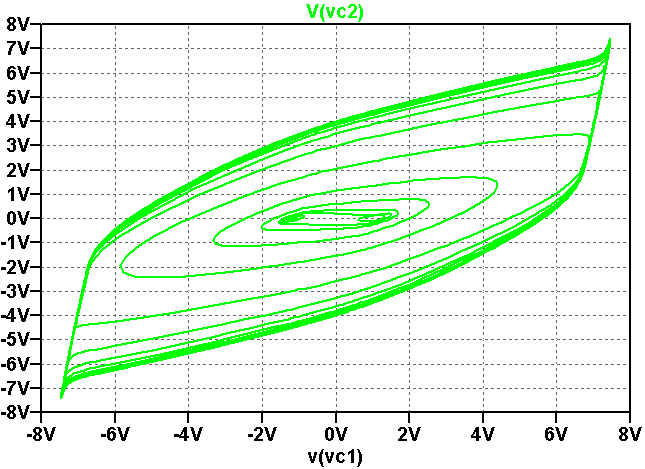
\includegraphics[width=5cm,height=5cm]{r0/ro1.png}&
        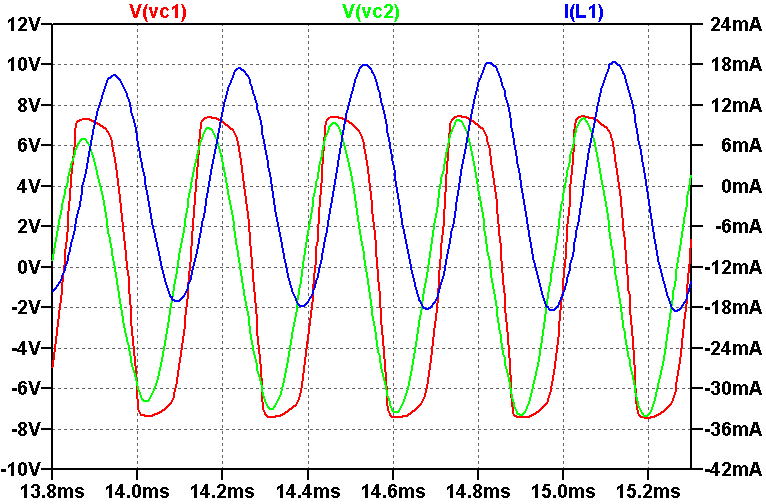
\includegraphics[width=5cm,height=5cm]{r0/ro1TS.png}&
        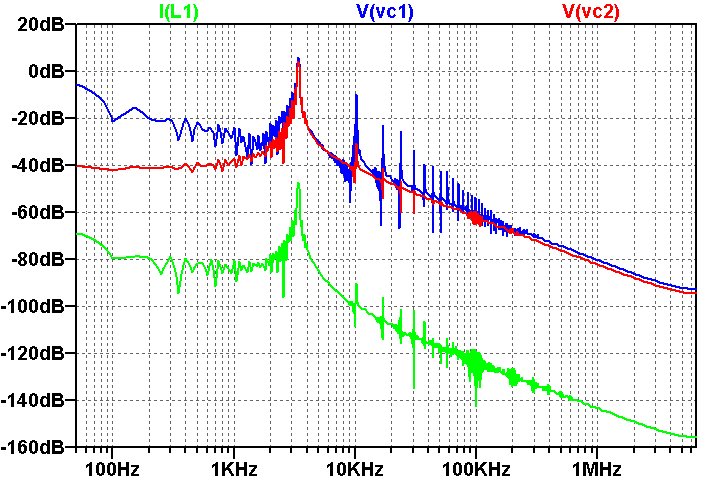
\includegraphics[width=5cm,height=5cm]{r0/ro1FFT.png}&\\
        & (1) & \\
        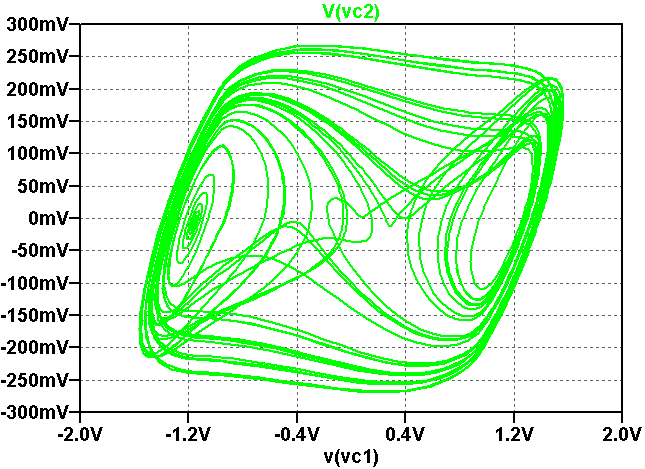
\includegraphics[width=5cm,height=5cm]{r0/ro10.png}&
        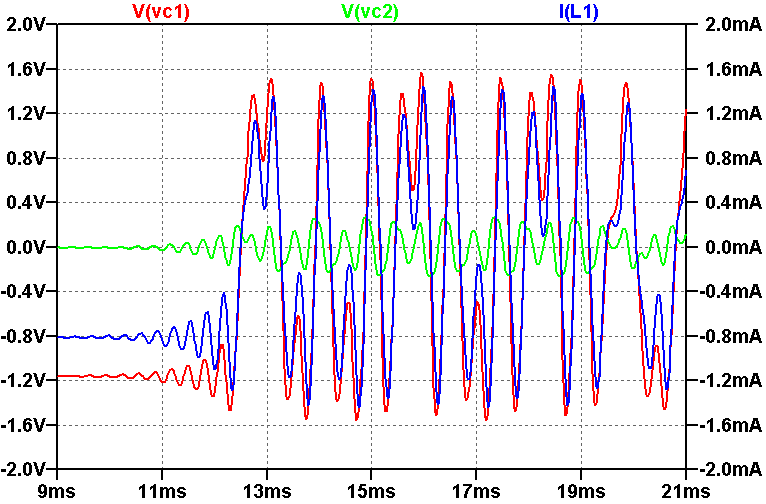
\includegraphics[width=5cm,height=5cm]{r0/ro10TS.png}&
        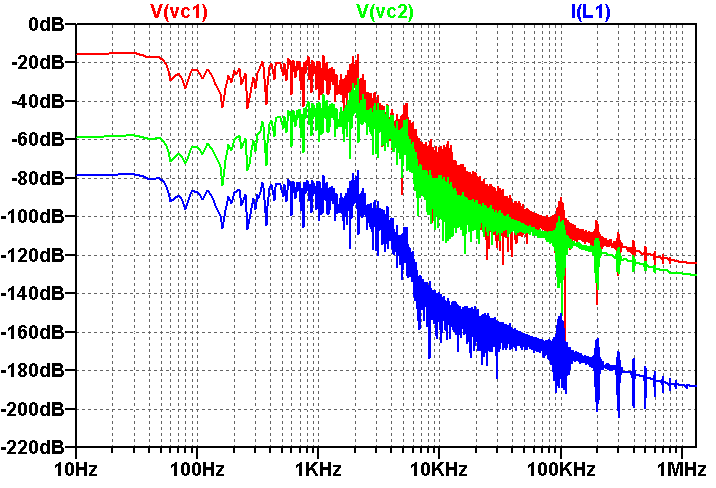
\includegraphics[width=5cm,height=5cm]{r0/ro10FFT.png}&\\
        & (2) & \\
        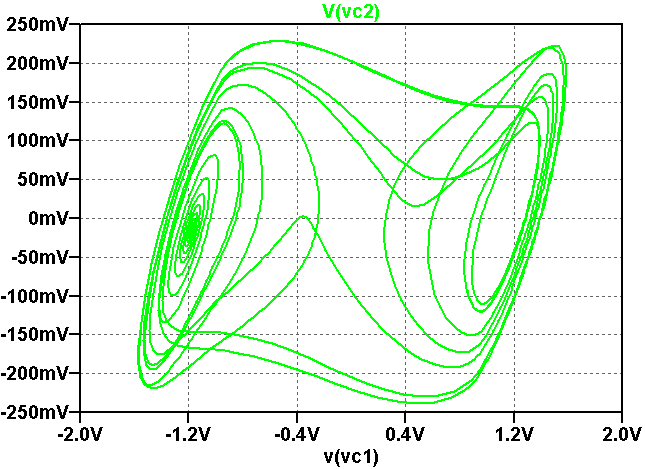
\includegraphics[width=5cm,height=5cm]{r0/ro20.png}&
        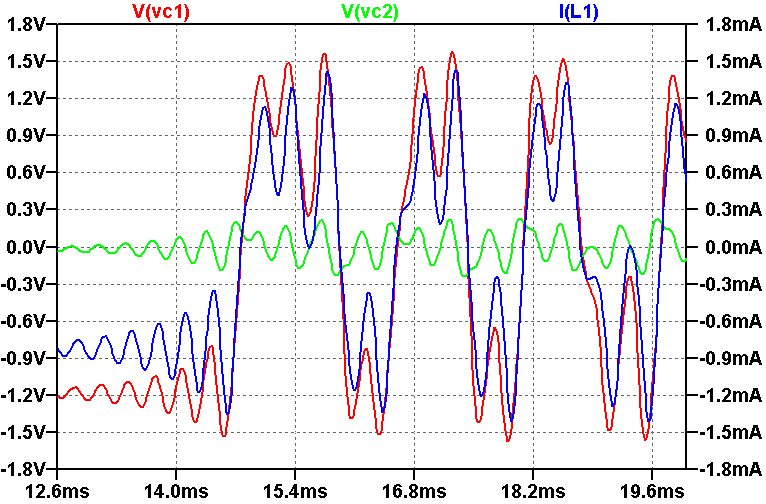
\includegraphics[width=5cm,height=5cm]{r0/ro20TS.png}&
        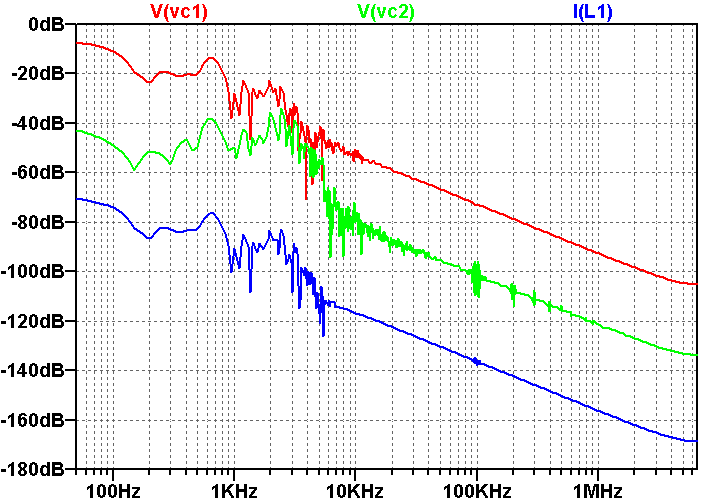
\includegraphics[width=5cm,height=5cm]{r0/ro20FFT.png}&\\
        & (3) &  \\
        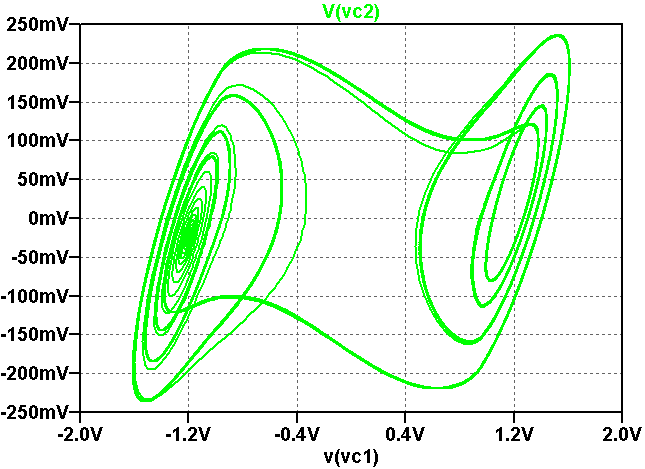
\includegraphics[width=5cm,height=5cm]{r0/ro30.png}&
        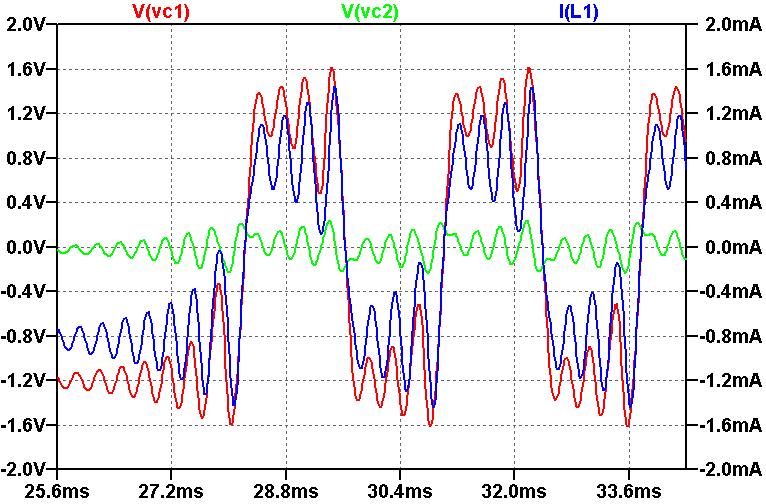
\includegraphics[width=5cm,height=5cm]{r0/ro30TS.png}&
        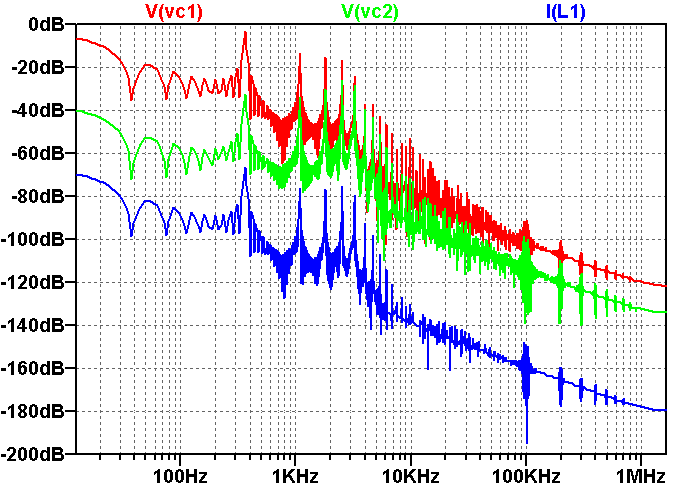
\includegraphics[width=5cm,height=5cm]{r0/ro30FFT.png}&\\
        & (4) &  \\
        \hline
    \end{tabular}
\end{table}
%TABLA 4
\begin{table}[h]
    \centering
        \caption{\label{tab:zzParámetro de control $r_0$ en el CCC}(continuación)}\\
        \begin{tabular}{c c c c}
        \hline
        \includegraphics[width=5cm,height=5cm]{r0/ro40_reg__TRAN_Y_EST_1_2.png}&
        \includegraphics[width=5cm,height=5cm]{r0/ro40TS.2.png}&
        \includegraphics[width=5cm,height=5cm]{r0/ro40_FFT.png}&\\
        & (5) &  \\  
        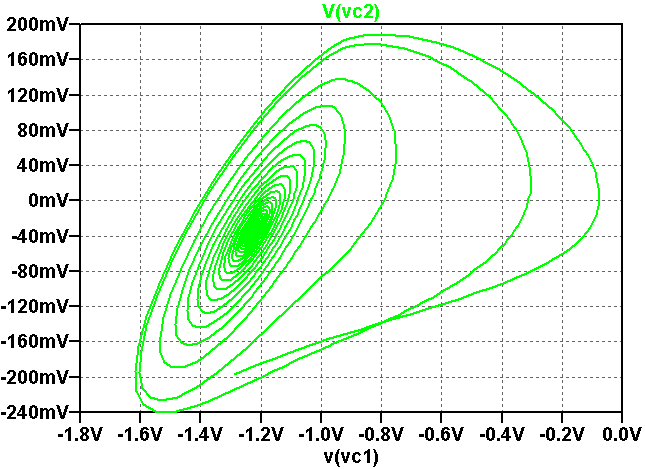
\includegraphics[width=5cm,height=5cm]{r0/ro40_reg_TRANS.png}&
        \includegraphics[width=5cm,height=5cm]{r0/ro40_reg_EST_1.png}&
        \includegraphics[width=5cm,height=5cm]{r0/ro40_reg_EST_2.png}&\\
        (6a) & (6b) & (6c) \\ 
        \includegraphics[width=5cm,height=5cm]{r0/ro40TS.1.png} & &
        \includegraphics[width=5cm,height=5cm]{r0/ro40_reg__EST_1_Y_2 ts.png}\\
        (7a) &  & (7b) \\
        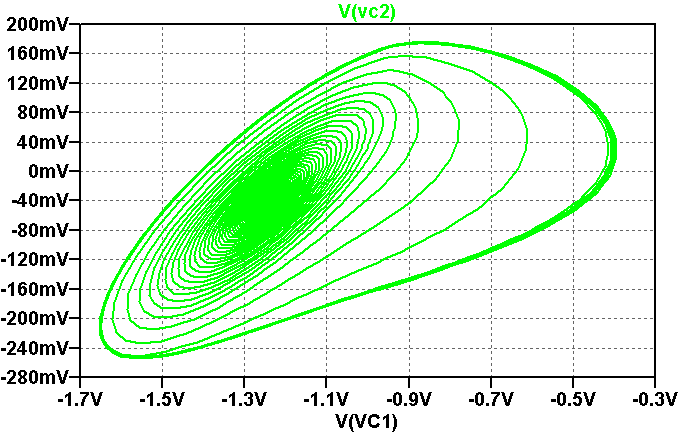
\includegraphics[width=5cm,height=5cm]{r0/ro50.png}&
        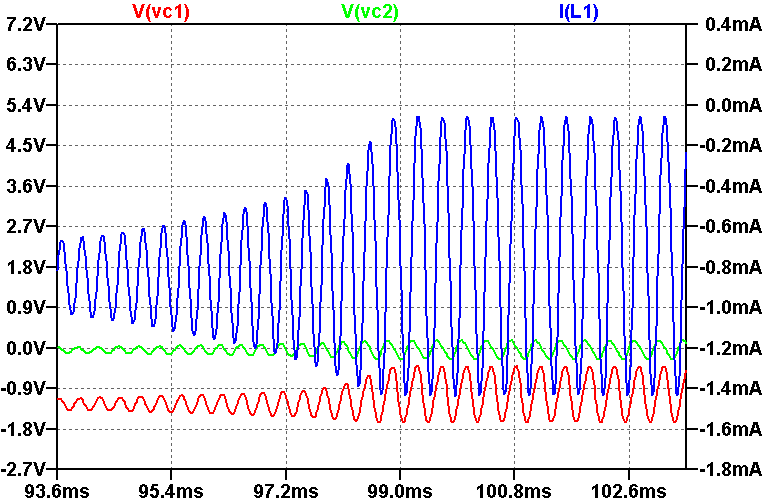
\includegraphics[width=5cm,height=5cm]{r0/ro50 ts.png}&
        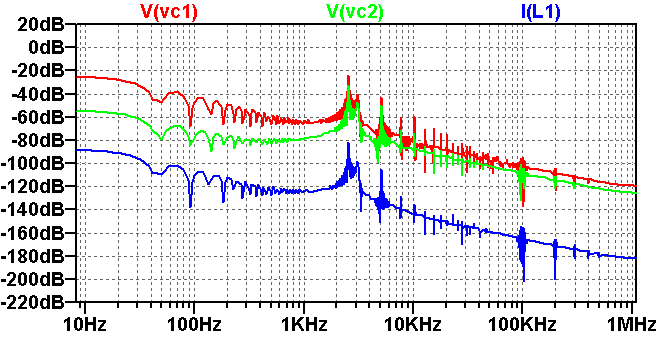
\includegraphics[width=5cm,height=5cm]{r0/ro50.FFT.png}&\\
        & (8) &  \\
        \hline
    \end{tabular}
\end{table}

%TABLA 5
\begin{table}[h]
    \centering
        \caption{\label{tab:CCC modificado variando r0}  Gráficas de $V_C1$, $V_C2$ e $I_L$, obtenidas en la simulación del CCC modificado variando r0, junto con sus series temporales y gráficos FFT.}\\
        \begin{tabular}{c c c c}
        \hline    
        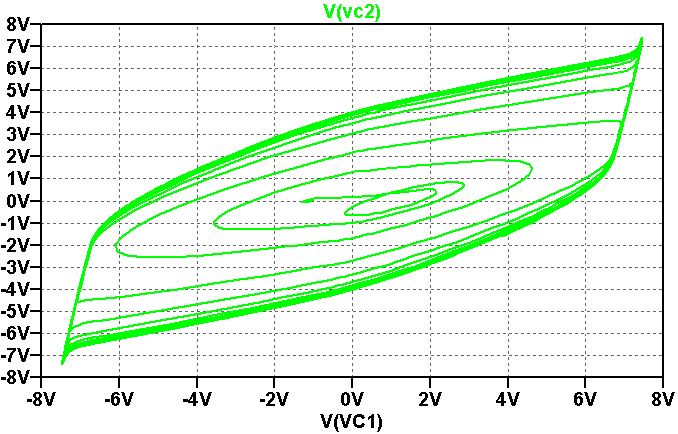
\includegraphics[width=5cm,height=5cm]{r0/ro1_cap.png}&
        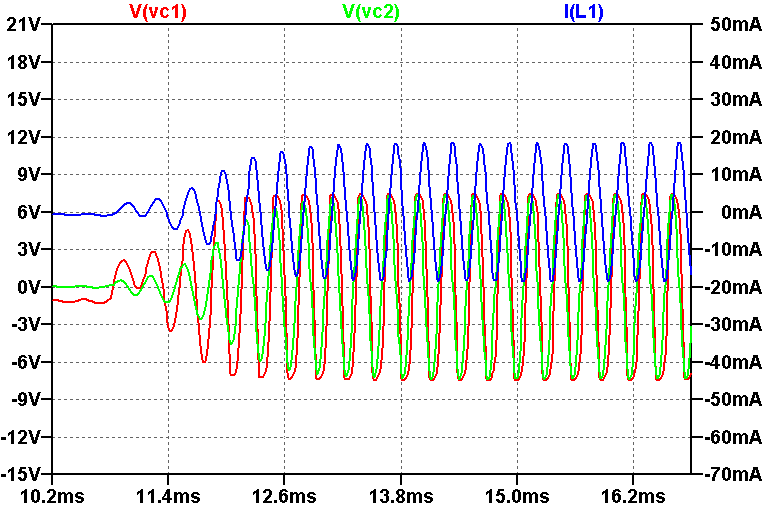
\includegraphics[width=5cm,height=5cm]{r0/ro1TS_cap.png}&
        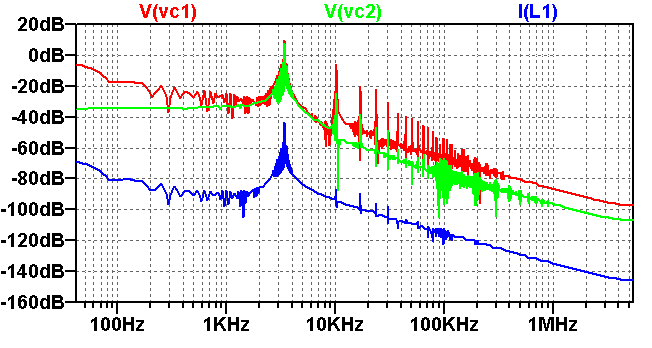
\includegraphics[width=5cm,height=5cm]{r0/ro1.FFT_cap.png}&\\
        & (1) & \\
        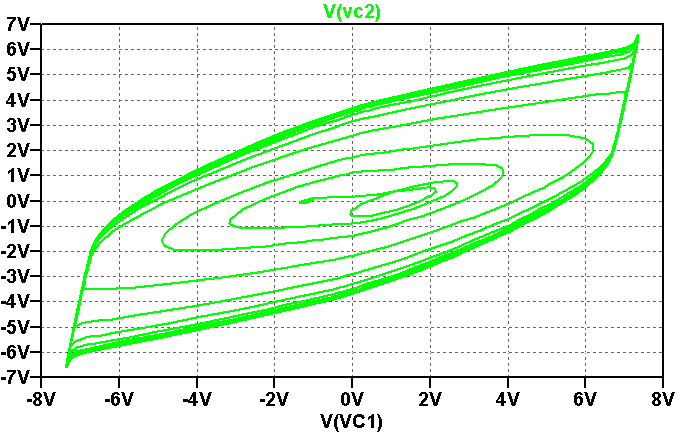
\includegraphics[width=5cm,height=5cm]{r0/ro10_cap.png}&
        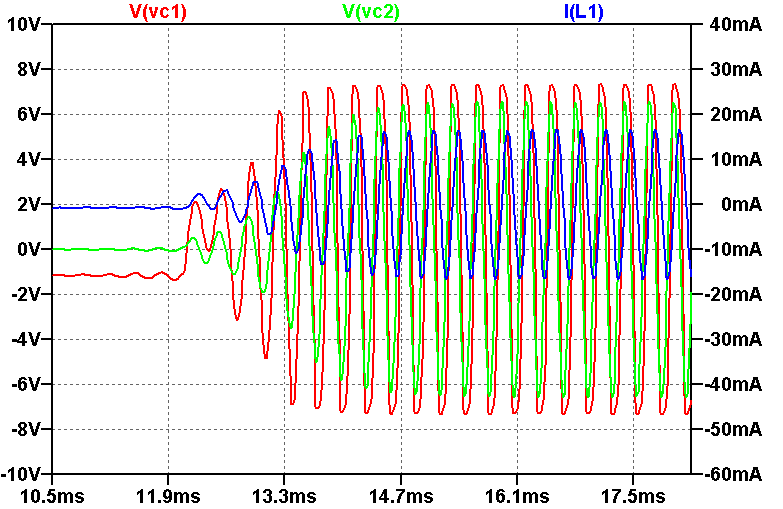
\includegraphics[width=5cm,height=5cm]{r0/ro10TS_cap.png}&
        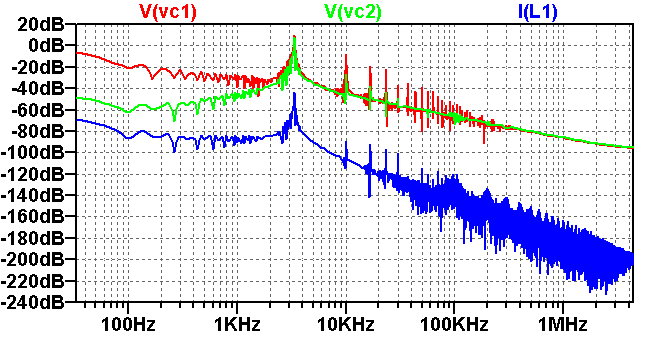
\includegraphics[width=5cm,height=5cm]{r0/ro10.FFT_cap.png}&\\
        & (2) & \\
        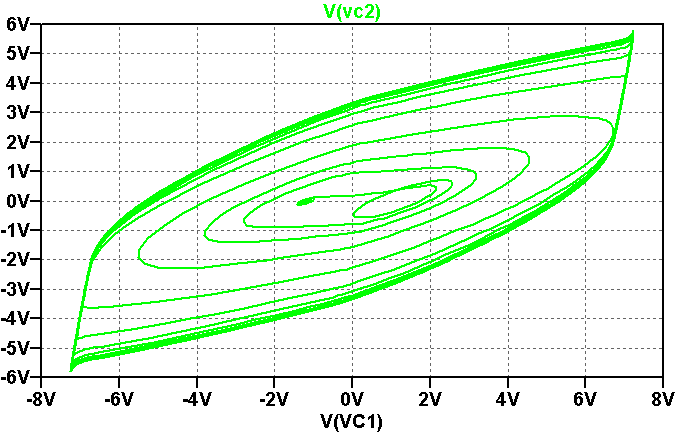
\includegraphics[width=5cm,height=5cm]{r0/ro20_cap.png}&
        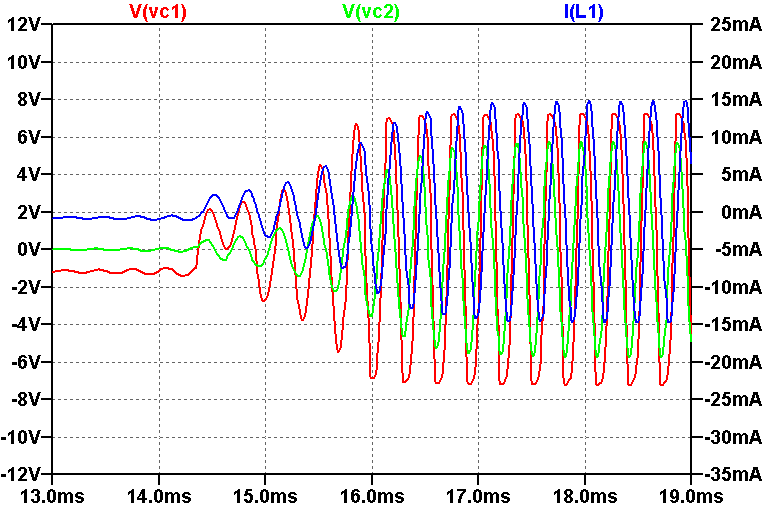
\includegraphics[width=5cm,height=5cm]{r0/ro20TS_cap.png}&
        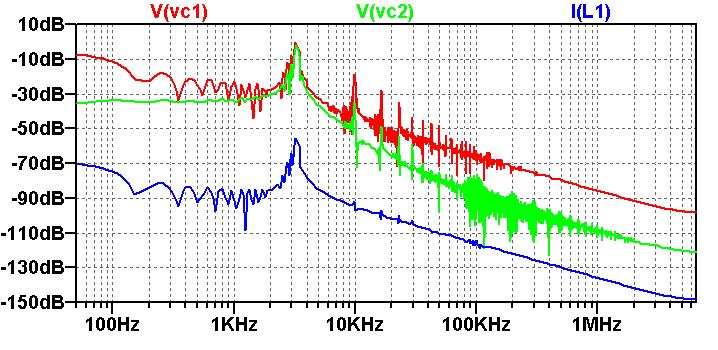
\includegraphics[width=5cm,height=5cm]{r0/ro20.FFT_cap.png}&\\
        & (3) & \\
        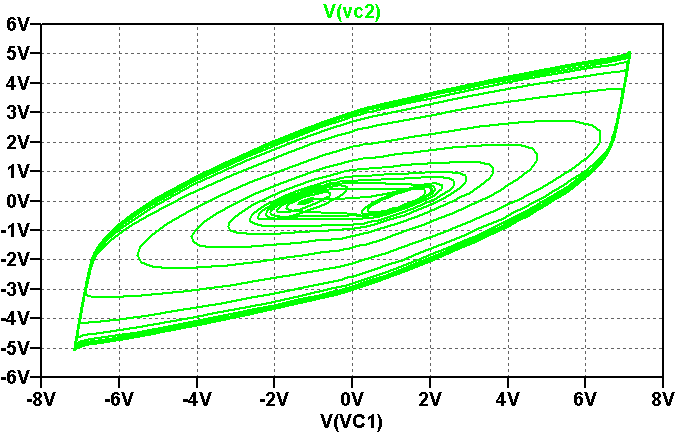
\includegraphics[width=5cm,height=5cm]{r0/ro30_Cap.png}&
        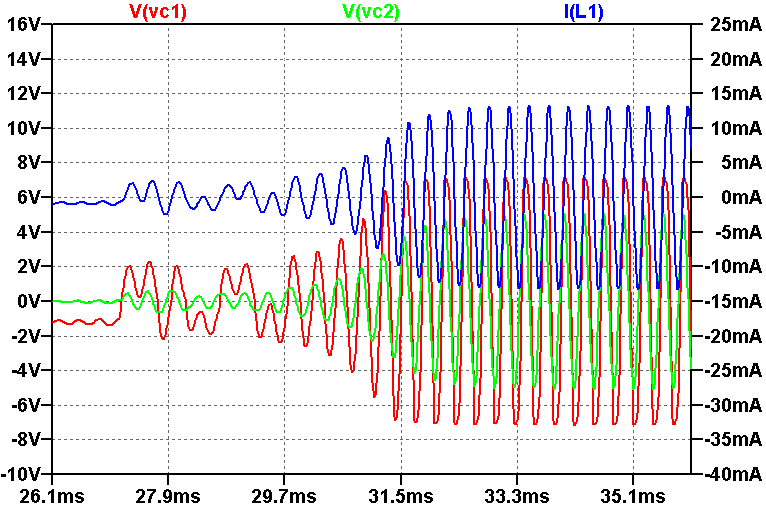
\includegraphics[width=5cm,height=5cm]{r0/ro30TS_Cap.png}&
        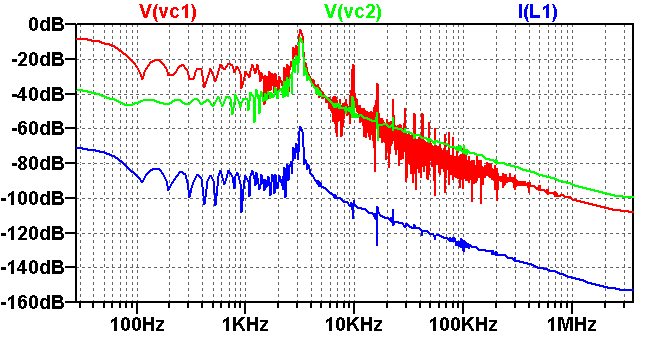
\includegraphics[width=5cm,height=5cm]{r0/ro30.FFT_Cap.png}&\\
        & (4) & \\
        \hline
    \end{tabular}
\end{table}
%TABLA 6
\begin{table}[h]
    \centering
    \caption{\label{tab:CCC modificado variando r0} (Continuación).}\\
    \begin{tabular}{c c c c}
        \hline    
        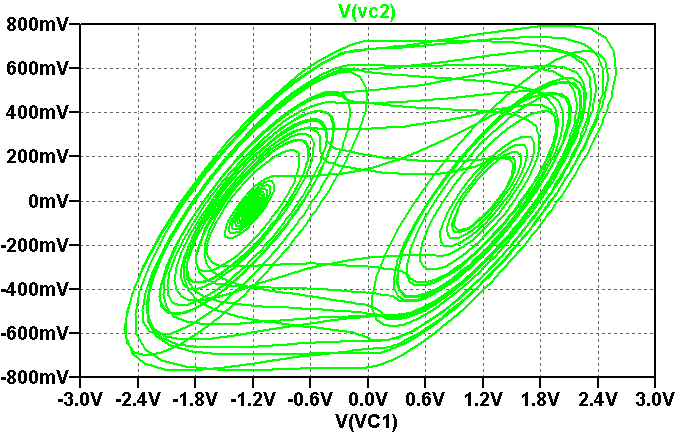
\includegraphics[width=5cm,height=5cm]{r0/ro40_transicion_cap.png}&
        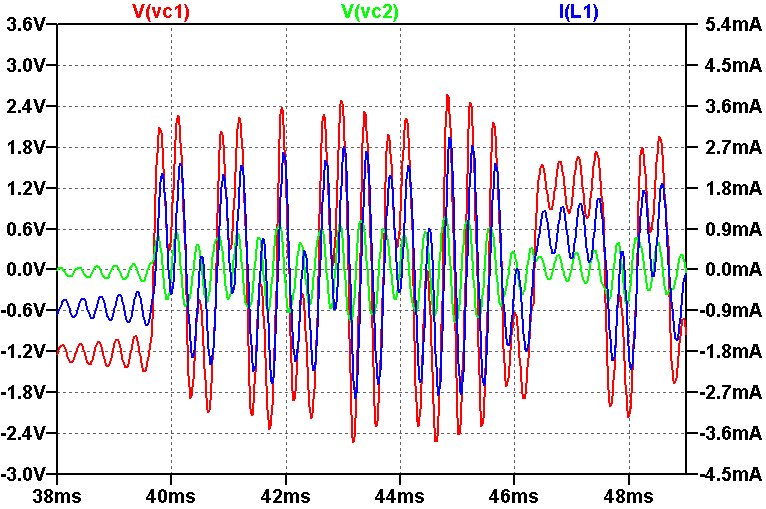
\includegraphics[width=5cm,height=5cm]{r0/ro40TS.1_transicion_cap.otra.png}&
        \includegraphics[width=5cm,height=5cm]{r0/ro40_FFT.png}&\\
        & (5) & \\   
        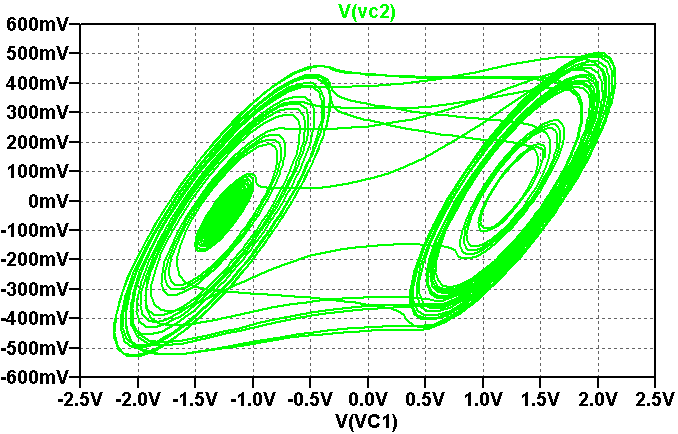
\includegraphics[width=5cm,height=5cm]{r0/ro50_CAP.png}&
        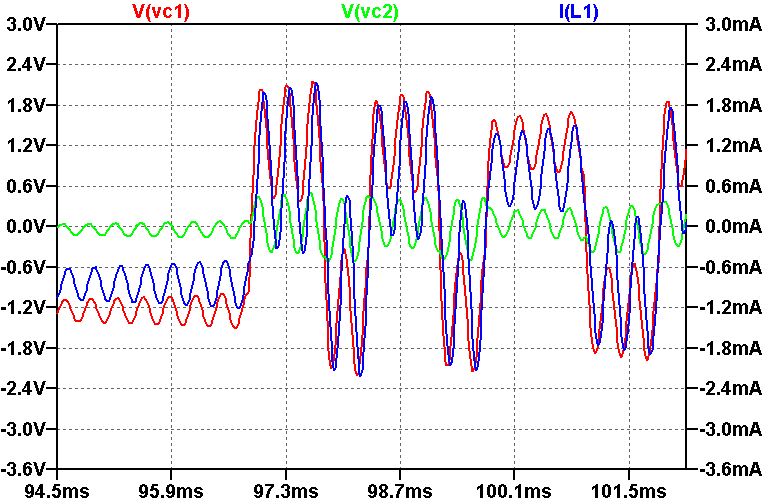
\includegraphics[width=5cm,height=5cm]{r0/ro50.TS_CAP.png}&
        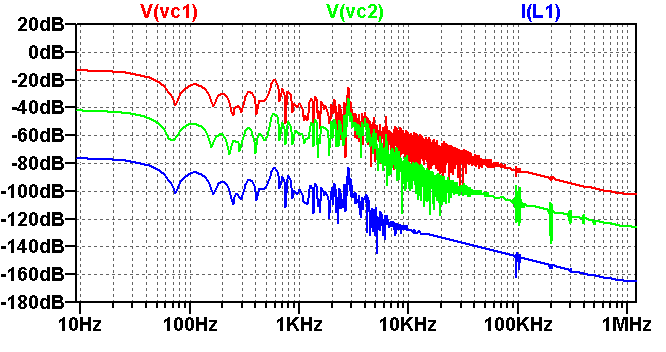
\includegraphics[width=5cm,height=5cm]{r0/ro50.FFT_CAP.png}&\\
        & (6) & \\   
        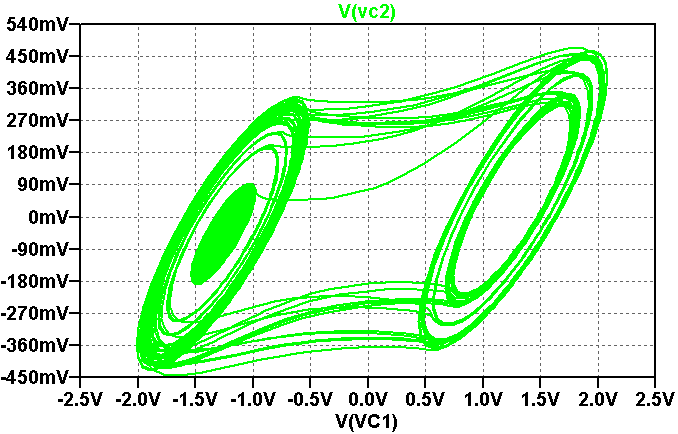
\includegraphics[width=5cm,height=5cm]{r0/ro56_CAP.png}&
        \includegraphics[width=5cm,height=5cm]{r0/ro56.TS_Cap.png}&
        \includegraphics[width=5cm,height=5cm]{r0/ro56.FFT_CAP.png}&\\
        & (7) & \\
        \hline
    \end{tabular}
\end{table}
%TABLA 7
\begin{table}[h]
    \centering
    \caption{\label{tab:$r_0$ fijo y variando R en el CCC} Gráficas de $V_C1$, $V_C2$ e $I_L$, obtenidas en la simulación del CCC variando R y $r_0$ fijo, junto con sus series temporales y gráficos FFT.}\\
        \begin{tabular}{c c c c}
        \hline    
        \includegraphics[width=5cm,height=5cm]{R7/1303 C0 atractor.png}&
        \includegraphics[width=5cm,height=5cm]{R7/1303 C0 ts.png}&
        \includegraphics[width=5cm,height=5cm]{R7/1303 C0 fft.png}&\\
        & (1) & \\
        \includegraphics[width=5cm,height=5cm]{R7/1379 C 0 720ms atractor.png}&
        \includegraphics[width=5cm,height=5cm]{R7/1379 C 0 720ms time series.png}&
        \includegraphics[width=5cm,height=5cm]{R7/1379 C 0 720ms fft.png}&\\
        & (2) & \\ 
        \includegraphics[width=5cm,height=5cm]{R7/1419 C0 ATRACTOR.png}&
        \includegraphics[width=5cm,height=5cm]{R7/1419 C0 TS.png}&
        \includegraphics[width=5cm,height=5cm]{R7/1419 C0 FFT.png}&\\
        & (3) & \\
        \includegraphics[width=5cm,height=5cm]{R7/1419.44 C0 800m atractor.png}&
        \includegraphics[width=5cm,height=5cm]{R7/1419.44 C0 800m time series.png}&
        \includegraphics[width=5cm,height=5cm]{R7/1419.44 C0 800m fft.png}&\\
        & (4) & \\
        \hline  
    \end{tabular}
\end{table}
%TABLA 8
\begin{table}[h]
    \centering
    \caption{\label{tab:r_0 fijo y variando R CCC modificado} Gráficas de $V_C1$, $V_C2$ e $I_L$, obtenidas en la simulación del CCC modificado usando R como parámetro de control y $r_0$=56 (\Omega) fijo, junto con sus series temporales y gráficos FFT.}\\
        \begin{tabular}{c c c c}
            \hline    
            \includegraphics[width=5cm,height=5cm]{R7/1303 C 220 attractor.png}&
            \includegraphics[width=5cm,height=5cm]{R7/1303 C 220 time series.png}&
            \includegraphics[width=5cm,height=5cm]{R7/1303 C 220 fft.png}&\\
            & (1) &  \\
            \includegraphics[width=5cm,height=5cm]{R7/1303 C 220 1ra EST 140ms atractor.png}&
            \includegraphics[width=5cm,height=5cm]{R7/1303 C 220 1ra EST 140ms time series.png}&
            \includegraphics[width=5cm,height=5cm]{R7/1303 C 220 1ra EST 140ms fft.png}&\\
            & (2) &  \\
            \includegraphics[width=5cm,height=5cm]{R7/1303 C 220 2do EST 200ms atractor.png}&
            \includegraphics[width=5cm,height=5cm]{R7/1303 C 220 2do EST 200ms time series.png}&
            \includegraphics[width=5cm,height=5cm]{R7/1303 C 220 2do EST 200ms time series.png}&\\
            & (3) &  \\
            \includegraphics[width=5cm,height=5cm]{R7/1379 C 220 210m atractor.png}&
            \includegraphics[width=5cm,height=5cm]{R7/1379 C 220 210m time series.png}&
            \includegraphics[width=5cm,height=5cm]{R7/1379 C 220 210m fft.png}&\\
            & (4) &  \\ 
            \hline  
       \end{tabular}
\end{table}
%TABLA 9
\begin{table}[h]
    \centering
    \caption{\label{tab:r_0 fijo y variando R CCC modificado}(Continuación).}
    \begin{tabular}{c c c c}
        \hline 
        \includegraphics[width=5cm,height=5cm]{R7/1419atractorC.png}&
        \includegraphics[width=5cm,height=5cm]{R7/1419tsC.png}&
        \includegraphics[width=5cm,height=5cm]{R7/1419fftC.png}&\\
        & (5) &  \\
        \includegraphics[width=5cm,height=5cm]{R7/1419.44 C220 800m atractor.png}&
        \includegraphics[width=5cm,height=5cm]{R7/1419.44 C220 800m time series.png}&
        \includegraphics[width=5cm,height=5cm]{R7/1419.44 C220 800m fft.png}&\\
        & (6) &  \\
        \includegraphics[width=5cm,height=5cm]{R7/1419.61 C220 800m atractor.png}&
        \includegraphics[width=5cm,height=5cm]{R7/1419.61 C220 800m time series.png}&
        \includegraphics[width=5cm,height=5cm]{R7/1419.61 C220 800m fft.png}&\\
     & (7) &  \\
     \hline  
    \end{tabular}
\end{table}
%TABLA 10
\begin{table}[h]
    \centering
    \caption{\label{tab:r_0 fijo y variando R CCC modificado} (Continuación).}\\
    \begin{tabular}{c c c c}
        \hline  
        \includegraphics[width=5cm,height=5cm]{R7/1419atractorC.png}&
        \includegraphics[width=5cm,height=5cm]{R7/1419tsC.png}&
        \includegraphics[width=5cm,height=5cm]{R7/1419fftC.png}&\\
        & (8) &  \\ 
        \includegraphics[width=5cm,height=5cm]{R7/1419.44 C220 800m atractor.png}&
        \includegraphics[width=5cm,height=5cm]{R7/1419.44 C220 800m time series.png}&
        \includegraphics[width=5cm,height=5cm]{R7/1419.44 C220 800m fft.png}&\\
        & (9) &  \\
        \includegraphics[width=5cm,height=5cm]{R7/1419.61 C220 800m atractor.png}&
        \includegraphics[width=5cm,height=5cm]{R7/1419.61 C220 800m time series.png}&
        \includegraphics[width=5cm,height=5cm]{R7/1419.61 C220 800m fft.png}&\\
        & (10) &  \\
        \hline  
    \end{tabular}
\end{table}

\section{resultados numéricos}
Para comparar los resultados de la simulación, se utilizo los valores de los componentes electrónicos de la Tabla \ref{tab:valores componentes electricos} y las ecs. \ref{alfa beta gamma}, para calcular todos los valores de las constantes involucradas en la ec. \ref{Chua eq dif} y se utiliza $\gamma$ como parámetro de control, usando los mismos valores de $r_0$ que se uso en las simulaciones. Estos valores se muestran en la Tabla \ref{tab:alfa b gamma calculados}, juntos con las condiciones iniciales que se utilizaron en las simulaciones, estas fueron sacadas de los datos de las series temporales.
Los comportamientos dinámicos obtenidos se muestran en la Tabla \ref{tab: imagenes numericas con valores calculados}, donde solo se ven comportamientos periódicos para los mismos valores usados de $r_0$ en la sección de simulado. Sin embargo, utilizando los valores clásicos de las pendientes internas y externas de la ec. \ref{f(x) PWL}, usados en Conde-Ramirez, et.al., se obtiene los comportamientos señalados en la Tabla\ref{} que muestra ciclos limites y un comportamiento caótico 1-scroll a primera vista, eventualmente podrían haber  mas comportamientos caóticos, pero para fines de este trabajo fue suficiente. Pues, es evidente que si se quiere empalmar con la parte experimental, se debe considerar cada mínimo detalle, detalles que en este trabajo fueron muchos y es evidente porque no se obtiene los mismos valores utilizados por la mayoría de investigadores, los convenios que se tuvieron a un inicio, claramente permanecen.

\begin{table}[h]
    \caption{\label{tab:alfa b gamma calculados} Valores de $r_0$, los correspondientes valores de \alpha, \beta y \gamma. Con sus respectivas condiciones iniciales.}
    \begin{ruledtabular}
    \begin{tabular}{c c c c c c c}
        $r_0$ (\Omega)  & \alpha & \beta & \gamma & x_0 & y_0 & z_0\\
        \hline
        1 & 10 & 11.18645 & 0.00788 & - 1.16357 & - 0.00814 & - 0.00081\\
        10 & 10 & 11.18645 & 0.07883 & - 1.16357 & - 0.00814 & - 0.00081\\
        40 & 10 & 11.18645 & 0.31533 & -1.22525 & - 0.03359 & -0.00084\\
        50 & 10 & 11.18645 & 0.39417 & -1.24661 & - 0.04243 & -0.00080\\
        56 & 10 & 11.18645 & 0.44147 & - 1.25963 & - 0.04782 & -0.00085\\
    \hline
    \end{tabular}
    \end{ruledtabular}
\end{table}

\begin{table}[h]
    \centering
    \caption{\label{tab: imagenes numericas con valores calculados} Los gráficos obtenidos mediante las ec. \ref{Chua eq dif}, usando la función del diodo de Chua aproximado con un polinomio cubico, usando el parámetro de control \gamma. Cada imagen esta enumerada en la parte inferior. Y los valores de $r_0$ usados estan dados en un recuadro dentro la misma imagen, como también sus condiciones iniciales. \\}
    \begin{tabular}{c c}
        \hline    
        \includegraphics[width=4.5cm,height=4.5cm]{Mat_r0_pwl_poly/phaseESPACEPolyr_01.png}
        \includegraphics[width=4.5cm,height=4.5cm]{Mat_r0_pwl_poly/timeseriesPolyr_01.png}&
        \includegraphics[width=4.5cm,height=4.5cm]{Mat_r0_pwl_poly/phaseESPACEPolyr_010.png}
        \includegraphics[width=4.5cm,height=4.5cm]{Mat_r0_pwl_poly/timeseriesPolyr_010.png}&
        (1) & (2) \\
        \includegraphics[width=4.5cm,height=4.5cm]{Mat_r0_pwl_poly/phaseESPACEPolyr_040.png}
        \includegraphics[width=4.5cm,height=4.5cm]{Mat_r0_pwl_poly/timeseriesPolyr_040.png}&
        \includegraphics[width=4.5cm,height=4.5cm]{Mat_r0_pwl_poly/phaseESPACEPolyr_050.png}
        \includegraphics[width=4.5cm,height=4.5cm]{Mat_r0_pwl_poly/timeseriesPolyr_050.png}&
        (3) & (4) \\
        \includegraphics[width=4.5cm,height=4.5cm]{Mat_r0_pwl_poly/phaseESPACEPolyr_056.png} &
        \includegraphics[width=4.5cm,height=4.5cm]{Mat_r0_pwl_poly/timeseriesPolyr_056.png}\\
        (5) \\
    \end{tabular}
\end{table}

\begin{table}[h]
    \centering
    \caption{\label{tab:parámetros de las pendientes clásicas de Conde-Rámirez} Gráficas obtenidas mediante las ec. \ref{Chua eq dif}, usando la función del diodo de Chua aproximada con un polinomio y \gamma como parámetro de control. Y usando los parámetros de las pendientes clásicas de Conde-Rámirez. Cada imagen contiende informacion de $r_0$ y las condiciones iniciales y su correspondiente numeración.\\}
    \begin{tabular}{c c}
        \hline    
        \includegraphics[width=4.5cm,height=4.5cm]{Mat_C_R_r0_poly1/phaseESPACEC_R_Polyr_01.png}
        \includegraphics[width=4.5cm,height=4.5cm]{Mat_C_R_r0_poly1/timeseriesC_R_Polyr_01.png}&
        \includegraphics[width=4.5cm,height=4.5cm]{Mat_C_R_r0_poly1/phaseESPACEC_R_Polyr_010.png}
        \includegraphics[width=4.5cm,height=4.5cm]{Mat_C_R_r0_poly1/timeseriesC_R_Polyr_010.png}&
        (1) & (2) \\
        \includegraphics[width=4.5cm,height=4.5cm]{Mat_C_R_r0_poly1/phaseESPACEC_R_Polyr_040.png}
        \includegraphics[width=4.5cm,height=4.5cm]{Mat_C_R_r0_poly1/timeseriesC_R_Polyr_040.png}&
        \includegraphics[width=4.5cm,height=4.5cm]{Mat_C_R_r0_poly1/phaseESPACEC_R_Polyr_050.png}
        \includegraphics[width=4.5cm,height=4.5cm]{Mat_C_R_r0_poly1/timeseriesC_R_Polyr_050.png}&
        (3) & (4) \\
        \includegraphics[width=4.5cm,height=4.5cm]{Mat_C_R_r0_poly1/phaseESPACEC_R_Polyr_056.png}&
        \includegraphics[width=4.5cm,height=4.5cm]{Mat_C_R_r0_poly1/timeseriesC_R_Polyr_056.png}\\
        (5) \\
    \end{tabular}
\end{table}

\subsection{Exponentes de Lyapunov y el parámetro d-infinito}

Para determinar que gráficas de la tabla \ref{tab:Parámetro de control $r_0$ en el CCC} son caóticas se utilizo el calculo de los exponentes de Lyapunov en Matlab con un tiempo de integración de 100. Se utilizan los mismos valores calculados de la Tabla \ref{tab:alfa b gamma calculados}. Y solo se utilizo $(\gamma)$ como parámetro de control.
Para realizar el calculo de los exponentes de Lyapunov, Se debe realizar una aproximación en la función lineal a tramos del diodo de Chua, ya que se tiene problemas con la derivada al momento de sacar el Jacobiano, en realidad, causa una acumulación de datos (ver anexos) al usar el algoritmo ode45 (Runge-Kutta (4,5)) en Matlab y para solventarlo se debe modificar el código, tal que, evite estos puntos ó, caso contrario, utilizar una función aproximada. En este caso se utilizo una aproximación para la ec.\ref{f(x) PWL} con un polinomio cubico, como detallan Ramírez & Gallas, Fig. \ref{PWL POLY}.
La Tabla \ref{tab:exponentes lyapunov con alfa beta calculados}, muestra los exponentes calculados, junto con los valores de las variables usadas. En la Fig. \ref{fig:Expo Lyap vs r0} se gráfica los exponentes de Lyapunov calculados.

\begin{figure}[h]
    \centering
    \includegraphics[width=7cm,height=7cm]{Mat_r0_pwl_poly/ChuasDIODES.png}
    \caption{Función PWL f y su aproximación con un polinomio cubico g en el intervalo [-2,2].}
    \label{PWL POLY}
\end{figure}

\begin{table}[h]
    \centering
    \caption{\label{tab:exponentes lyapunov con alfa beta calculados}Exponentes Lyapunov para el CCC con \gamma como parámetro de     control.} 
    \begin{tabular}{c|c|c|c|c|c|c|c|c}
    r0(\Omega)	& gamma	& x0	& y0	& z0	& \lambda_1 & \lambda_2 & \lambda_3\\ 
    \hline  
    1& 56	& 0.44147 & -1.25963 & -0.04782 & -0.00085 & 0.016871 & -0.131181 & -7.071438\\	 
    2& 50	& 0.39417 & -1.24661 & -0.04243 & -0.00080	& 0.004856 & -0.188533 & -7.802514\\
    3& 40	& 0.31533 & -1.22525 & -0.03359 & -0.00084 	& -0.024541 & -0.258835 & -9.043396\\			 
    4& 10 & 0.07883 & -1.16357	& -0.00814 & -0.00081 & -0.146213 & -0.402821 & -13.482867\\
    5& 1	& 0.00788 & -1.16357 & -0.00814 & -0.00081 & -0.188466 & -0.429689 & -15.154892\\
    \end{tabular}
\end{table}

\begin{figure}
    \centering
    \includegraphics[width=7.5cm,height=7.5cm]{Lyap_t_trans_d/Lyapunov_r_056.png}\\
    (a)\\
    \includegraphics[width=7.5cm,height=7.5cm]{Lyap_t_trans_d/r_0_vs_Exp_Lyapunov_x_y_z.png}\\
    (b)\\
    \caption{ Exponentes de Lyapunov de la tabla \ref{tab:exponentes lyapunov} del CCC para: (a) el caso $r_0=56 \Omega$ donde la linea roja es \lambda_1, verde \lambda_2 y azul \lambda_3. Y en (b) se gráfica vs. $r_0$.}
    \label{fig:Expo Lyap vs r0}
\end{figure}
        
El mayor exponente de Lyapunov cuantifica el efecto del fenómeno de estiramiento en un sistema caótico. Sin embargo, en lo que respecta al plegamiento, necesitamos un parámetro más. Para ello, consideremos la siguiente ecuación :

\begin{equation}\label{d-infinito}
    d/dt d(t) & = \lambda_{1}d(t) - (\Gamma)d(t)^2\\
\end{equation}

donde d(t) representa la distancia entre dos trayectorias del mismo sistema dinámico que parten de dos condiciones iniciales diferentes, $\lambda_1$ es el mayor exponente de Lyapunov y $\Gamma$ es un parámetro que explica el fenómeno de plegamiento. La tendencia de d(t) es peculiar cuando se calcula para un sistema caótico: inicialmente, aumenta con una pendiente igual a $\lambda_1$ hasta que alcanza un valor estacionario alrededor del cual fluctúa. Este valor estacionario se denomina d-infinito ($d_∞$) y puede estimarse como λ1/$\Gamma$. La estimación del parámetro $d_∞$ nos permite también discernir entre el caos determinista y el ruido aleatorio. Para calcular la tendencia de d(t) se utilizo la metodología descrita en Thompson–Steward y adaptada a Matlab, esto se muestra en la Fig. \ref{fig:d infinito} para el caso de $r_0=56\Omega$.

\begin{figure}
    \centering
    \includegraphics[width=7.5cm,height=7.5cm]{Lyap_t_trans_d/d_infinito_r_50.png}
    \caption{Parámetro d-infinito para el caso de $r_0 = 58 {\Omega}$.}
    \label{fig:d infinito}
\end{figure}

%{Resultados de los circuitos físicos}
La tabla \ref{circuitos físicos} muestra los comportamientos obtenidos en el CCC modificado físico, usando el parámetro de control R. La Tabla \ref{datos osciloscopio} muestra los datos del circuito a través de un osciloscopio.
\begin{table}[h]
    \centering
    \caption{\label{circuitos físicos} 
    Comportamientos obtenidos en del circuito de Chua físico. Cada imagen esta con su correspondiente numeración.\\}
    \begin{tabular}{c c c c}
    \hline    
    \includegraphics[width=4.5cm,height=4.5cm]{Fotos_Chua_Experimentales/Chua1.jpg}&
    \includegraphics[width=4.5cm,height=4.5cm]{Fotos_Chua_Experimentales/Chua2.jpg}&
    \includegraphics[width=4.5cm,height=4.5cm]{Fotos_Chua_Experimentales/Chua3.jpg}&
    \includegraphics[width=4.5cm,height=4.5cm]{Fotos_Chua_Experimentales/Chua4.jpg}&
    (1) & (2) & (3) & (4)\\
    \includegraphics[width=4.5cm,height=4.5cm]{Fotos_Chua_Experimentales/Chua5.jpg}&
    \includegraphics[width=4.5cm,height=4.5cm]{Fotos_Chua_Experimentales/Chua6.jpg}&
    \includegraphics[width=4.5cm,height=4.5cm]{Fotos_Chua_Experimentales/Chua7.jpg}&
    (5) & (6) & (7) &\\
    \end{tabular}
\end{table}
Gráficas obtenidas con datos de osciloscopio del circuito de Chua modificado.
\begin{table}[h]
    \centering
    \caption{\label{datos osciloscopio} 
    Comportamientos obtenidos mediante los datos de un osciloscopio del circuito de Chua modificado. Cada imagen esta con su correspondiente numeración.\\}
    \begin{tabular}{c c c c}
    \hline    
    \includegraphics[width=4.5cm,height=4.5cm]{imagenesDATOS/data01.png}&
    \includegraphics[width=4.5cm,height=4.5cm]{imagenesDATOS/data02.png}&
    \includegraphics[width=4.5cm,height=4.5cm]{imagenesDATOS/data03.png}&
    \includegraphics[width=4.5cm,height=4.5cm]{imagenesDATOS/data04.png}&
    (1) & (2) & (3) & (4)\\
    \includegraphics[width=4.5cm,height=4.5cm]{imagenesDATOS/data05.png}&
    \includegraphics[width=4.5cm,height=4.5cm]{imagenesDATOS/data06.png}&
    \includegraphics[width=4.5cm,height=4.5cm]{imagenesDATOS/data07.png}&
    \includegraphics[width=4.5cm,height=4.5cm]{imagenesDATOS/data08.png}&
    (5) & (6) & (7) & (8)\\
    \includegraphics[width=4.5cm,height=4.5cm]{imagenesDATOS/data09.png}&
    \includegraphics[width=4.5cm,height=4.5cm]{imagenesDATOS/data10.png}\\
    (9) & (10)\\
    \end{tabular}
\end{table}

\section{Conclusiones y perspectivas}
Mediante las series temporales, para el caso de la simulación, se pudo ver si nuestro circuito reproducirá experimentalmente los atractores de Chua, pues cuando las configuraciones, son tales, que no se pasa la región transitoria y no se llega a la región estable, los atractores no se obtienen y solo se manifiestan efectos del transitorio, como se muestra en las  gráficas de las simulaciones. Para un valor bajo de resistencia interna, la región estable se alcanza en un menor tiempo de simulación  como se ve en la Tabla \ref{tab:r0 regimen transitorio y estable} y esto influye en gran medida que los comportamientos caóticos se puedan presentar cuando se utiliza valores elevados de la resistencia interna del inductor.
Se pudo verificar mediante simulaciones que los resultados experimentales de la Tabla \ref{datos osciloscopio} son reproducibles, por lo que, se asume que la modificación en el diodo de Chua en efecto tiene una riqueza dinámica que aun falta mucho por explorar debido a que no se encontró investigaciones que ya hayan trabajado exactamente con este modificación en el diodo de Chua.

Varias cosas estudiadas están en concordancia con los resultados de Conde & Ramírez, fueron de mucha utilidad, ya que ayudo a corroborar y entender varios resultados encontrados.

La comparación de las características físicas del modelo de Chua con el modelo modificado muestran que las ecuaciones modificada conllevan una mayor complejidad por lo que se espera que la riqueza en cuanto a su comportamiento dinámico sea mayor, debido a su comportamiento histerético, como pasa en el circuito de Saito. Lo que constituye un desafío para futuras investigaciones.
Por un lado, luego de darle el formalismo electrónico necesario, se puede proceder a realizar todos los estudios que hasta hoy se han hecho al circuito de Chua. Y por otro, independientemente de este formalismo se pueden realizar, los cálculos de:

- Exponentes de Lyapunov usando los datos usando Tisean.
- Mapa de bifurcaciones. 
- El espacio de parámetros como se realiza en Conde & Ramírez y ver si se manifiestan los camarones de Gallas & Ramírez.
- El modelado matemático de la histéresis, que modificara la función PWL del diodo de Chua.
-seguir investigando el fenómeno de histéresis, como lo hace Chua &  con otros componentes resistencias, inductancias, etc. 
\begin{acknowledgments}
Agradezco enormemente a la comunidad de investigadores apasionados de la carrera de Física por haber permitido, ayudado, motivado de una u otra manera desde el área en la que se desenvuelven a realizar el presente trabajo.
\end{acknowledgments}

\appendix

\nocite{*}
\bibliography{rbf}% Produce las referencias via BibTeX.
\end{document}
%
% ****** Fin del archivo rbf.tex ******
